% !TEX root = TD_fluides_part1_2018.tex

\section{Hydrostatique}


\setcounter{subsection}{-1}
\subsection{$^*$ Forces de pression sur un barrage}

%\begin{figure}[H]
%\includegraphics[width=\linewidth]{Biplan.eps}
\input{BarrageTriangulaire.pstex_tm} 
%\end{figure}

On considère un lac dans une vallée de section triangulaire,
d'angle au sommet $2\alpha$.
Le lac est fermé par un barrage de hauteur 
$h$. Le lac est rempli
d'eau de densité constante $\rho$, et sa surface est à la pression 
atmosphérique $P_a$.


\begin{enumerate}

\item Donnez l'expression de la pression $P(z)$ régnant dans le lac, où $z$ est l'altitude 
comptée par rapport à la base du barrage.

\item Calculez la résultante $\vec R$ des forces de pression exercées par l'eau 
et par l'air sur la surface du barrage.

\item Calculez le moment $\vec{\mathcal M}_O$ des forces de pression par
rapport au point $O$.

\item Donnez la position du centre de poussée $F$ des forces de pression.

\end{enumerate}



\subsection{Modèle d'atmosphère normalisée}

Le {\em modèle d'atmosphère normalisée }  ( \verb| http://fr.wikipedia.org/wiki/Atmosphère_normalisée | )
est un modèle adopté internationalement qui découpe l'atmosphère en sept couches successives
dans lesquelles la température est donnée par une loi affine de la forme 
$$T(z) = T_0 ( 1 - \alpha z)$$

On considère ici uniquement la couche inférieure appelée troposphère ($0<z<11km$) dans laquelle
les paramètres de cette loi sont  $\alpha = 22.6 \cdot 10^{-6} m^{-1}$ et $T_0 = 288 K$.  

Donnez les loi $P(z)$ et $\rho(z)$ correspondantes, sachant que la pression au niveau du sol
est $P_0 = 1013 hPa$.

\subsection{La montgolfière}

On considère une montgolfière, constituée d'un ballon sphérique et de 
rayon $R = 8m$, ouvert à sa base par une ouverture de section négligeable, et d'une nacelle.

On souhaite déterminer la température à laquelle il faut chauffer le gaz intérieur
pour pouvoir voler à l'altitude de $h=1000m$.

\begin{enumerate}

\item En utilisant le modèle d'atmosphère standard, donnez la masse volumique 
$\rho_{ext}$, la température $T_{ext}$ et la pression $P_{ext,h}$ caractérisant l'air à l'extérieur 
de la montgolfière à l'altitude $h = 1000m$ correspondant à la base du ballon.

\item
Quelle erreur commet-on en supposant la masse volumique constante à l'échelle du ballon ? 
Montrez que dans cette approximation la pression peut être approximée par une loi affine
de la forme $P_{ext}(z') \approx P_{ext,h}+a z'$ où $z' = z-h_0$ est l'altitude comptée à partir
de la base du ballon.


\item Le ballon est rempli d'air de masse volumique $\rho_{int}$ supposée uniforme.
Donnez la loi de pression $P_{int}(z')$ à l'intérieur du ballon.

\item Calculez la résultante des efforts exercés par l'air sur le ballon.

\item Retrouvez le résultat précédent à l'aide du théorème d'Archimède.

\item Application : calculez la valeur de $\rho_{int}$ nécessaire pour 
maintenir la montgolfière en équilibre à l'altitude 1000m, considérant que 
sa masse totale est $m=2500kg$. En déduire la température $T_{int}$
mesurée à la base du ballon.

\end{enumerate} 




  
\subsection{Envasement d'une barge}


%\begin{figure}[H]
%\includegraphics[width=\linewidth]{Biplan.eps}
\input{BargeVase.pstex_tm} 
%\end{figure}
  
On considère une barge de section carrée, de largeur $b=10m$ de hauteur 
$h=1m$,  et de masse $M = 75 t$. 
La barge flotte dans de l'eau de densité $\rho_e=1000kg m^{-3}$.
A marrée haute la hauteur d'eau est $H > h$.
  
  
\begin{enumerate}

\item Calculez le tirant d'eau de la barge à marée haute.


\item A marée basse la hauteur d'eau est de $H =25cm$, et la barge
s'enfonce dans la vase, que l'on considère comme un fluide de masse volumique
$\rho_v = 2 \rho_e$.
Calculez la profondeur d'envasement $e$.

\item Calculez l'allègement qu'il faudrait faire subir à la barge pour éviter
son envasement.


\end{enumerate}  


\subsection{$*$ Lois de pression et de température en fonction de la profondeur}

On cherche à estimer les lois de pression $P(z)$ et de 
masse volumique $\rho(z)$ dans l'océan en fonction de la profondeur $z$.
Les altitudes $z$ sont comptées vers le bas à partir de la surface
de l'océan, et la pression au niveau de la mer est $P_0 = 1,013 Bars$.

On donne les informations suivantes :

\begin{itemize}

\item La couche superficielle, qui s'étend jusqu'à environ 500 mètres de 
profondeur, est appelée thermocline. Dans cette couche la température
varie entre $T = 25^o C$ (en surface) et $T = 1.5^o C$ (à la base de la
thermocline). On suppose pour simplifier que la salinité est constante ($S = 35g/kg$).

On supposera que dans la thermocline la compressibilité est négligeable, de sorte que 
la masse volumique dépend seulement de la température, et est donnée par la relation 
simplifiée suivante (issue de l'équation d'état officielle IES80, avec $T$ en $^o C$, $\rho$ en $kg/m^3$ ) :
$$ 
\rho = 1028.15 - 0.05403 \times T - 0.006762\times  T^2 +7.955\cdot 10^{-5} \times T^3 - 9.3152 \cdot 10^{-7} \times T^4
+ 6.5363  \cdot 10^{-9}  \times T^5.
$$


%$\rho$ évolue notablement, principalement 
%sous l'effet de variations de température et de salinité.
%Plus précisément, la masse volumique passe de $\rho_0 = 1023 kg m^{-3}$
%en surface $(z=0)$, à la valeur $\rho_1 = 1030 kg m^{-3}$ à la profondeur
%$z_1 = 500 m$. 
%A la base de celle-ci 
%la température est $T_1 = 1.5 ^o C$.


\item Dans les couches plus profondes,  à cause de la compressibilité de l'eau de mer, la masse volumique et la température varient (faiblement) en fonction de la pression.

On supposera que dans les couches profondes les coefficients
thermodynamiques et thermoélastiques sont constants, et ont les valeurs suivantes :

$$
\chi_s = 4.6 \cdot 10^{-10} Pa^{-1} ; \quad 
\alpha_p = 8 \cdot 10^{-5} K^{-1} ; \quad 
c_p = 4000 J \cdot K^{-1} \cdot kg^{-1}.  
$$

%où $\rho_1$ et $P_1$ sont les valeurs à la base de la thermocline, 
%et $K$ est un "coefficient d'élasticité", 
%supposé constant, qui vaut :

%$$
%K = 23000 Bars.
%$$

%$$
%\chi = \frac{1}{\rho} 
%{\left(\frac{\partial \rho}{\partial p}\right)}_{T,S} = 4,5 \times 10^{-10} 
%Pa^{-1}.
%$$




\end{itemize}

\begin{enumerate}

\item Donnez la masse volumique en surface ($\rho_0$) et à la base de 
la thermocline ($\rho_1$). En déduire la loi de masse volumique $\rho(z)$  
dans la thermocline, en supposant qu'elle varie linéairement avec la profondeur.

\item  Déduisez-en la loi de pression $P(z)$ dans la thermocline.
Donnez en particulier la pression $P_1$ à la base de la thermocline. 


\item Dans les couches profondes, la masse volumique peut s'exprimer 
en bonne approximation par l'équation linéaire suivante :
$$
\rho = \rho_1 \left( 1 + \chi_s (P-P_1) \right).
$$ 
Donnez les lois de pression $P(z)$  et de masse volumique dans les 
couches profondes de l'océan ($z>z_1$). 
Donnez une approximation polynômiale de ces lois sous la forme
 $P(z) = P_1 + a (z-z_1)+ b (z-z_1)^2$, et $\rho(z) = \rho_1 + c (z-z_1)$.

\item 
Démontrez la relation suivante entre les coefficients thermodynamiques : 
$$
\epsilon_s = \frac{1}{T}
{\left(\frac{\partial T}{\partial  P}\right)}_{s} = \frac{\alpha_p}{\rho c_p}
$$

\item Déduisez-en la loi de température $T(z)$ dans les couches profondes $(z>z_1)$.


\item Application. La fosse océanique la plus profonde sur terre est située dans le 
Pacifique, au large de l'archipel des Mariannes, 
et atteint la profondeur $z=11000 m$. 
Donnez la pression (en bars), la masse volumique et la température 
reignant à cette profondeur.

%Quelle erreur aurait été commise sur la pression calculée précédemment 
%si on avait supposé la masse volumique de l'eau constante, 
%de valeur $\rho = 1030 kg m^{-3}$ ?

%\item Montrez que dans les couches profondes, 
%la loi de masse volumique calculée précédemment peut être remplacée
%en première approximation par une loi linéaire 
%de la forme $\rho = \rho_1 + A(z-z_1)$, et la loi de pression par une loi
%quadratique de la forme $P = P_1+B(z-z_1)+C(z-z_1)^2$.
%Donnez l'erreur commise en faisant cette approximation pour la profondeur 
%de la fosse des Mariannes.
\end{enumerate}

%\clearpage





\Archives{

\centerline{\fbox{\textbf{\Large Thème 1 : Statique des fluides}}}

\vspace{.5cm}


%%%%%%%%%%%%%%%%%%%%%%%%%%%%%%%%%%%%%%%%%%%%%%%%%%%%%%%%%%%%%%%%%%%%%%%%%%%%%%%
\subsection{Modèles d'atmosphère}
%%%%%%%%%%%%%%%%%%%%%%%%%%%%%%%%%%%%%%%%%%%%%%%%%%%%%%%%%%%%%%%%%%%%%%%%%%%%%%%

L'atmosphère est constitué d'air, considéré comme un gaz parfait avec $ r = 287 J/K/kg$.
Au sol ($z=0$), on a une temp\'erature $T_0 = 288$ K et une pression
$P_0 = 1.013 \; 10^5$ Pa. 

D\'eterminer la loi de pression $P(z)$ en fonction de l'altitude $z$
pour les trois modèles suivants :
\begin{enumerate}
\item
Atmosphère isotherme~: $T(z) = T_0$.
\item
Atmosphère adiabatique : pression et masse volumique sont reliés par
une relation de la forme $p \rho ^{-\gamma} = cte$.

\item 
Atmosphère "standart", c'est à dire dont la température varie selon la loi 
$T(z) = T_0 (1 - \alpha z)$ avec $\alpha = 22.6 \; 10^{-6}$m$^{-1}$ pour $0<z<11 km$,
et est constante, avec la valeur $T = T_1 = 216,4 K$, au delà de cette altitude
(modèle adopté au cours d'une conférence internationale d'aéronautique en 1910)

\end{enumerate}
Pour chaque cas, on calculera la pression au sommet de l'Everest ($z = 8848 m$), 
à l'altitude de vol du Concorde ($z=20km$).




%%%%%%%%%%%%%%%%%%%%%%%%%%%%%%%%%%%%%%%%%%%%%%%%%%%%%%%%%%%%%%%%%%%%%%%%%%%%%%%
\subsection{Distribution de pression dans les oc\'eans}
%%%%%%%%%%%%%%%%%%%%%%%%%%%%%%%%%%%%%%%%%%%%%%%%%%%%%%%%%%%%%%%%%%%%%%%%%%%%%%%

L'eau de mer a une concentration en sel et une temp\'erature 
qui varient suivant la profondeur,
ce qui conduit \`a une masse volumique non homog\`ene dans le fluide
(\textsl{stratification}) que l'on peut mod\'eliser par la loi lin\'eaire~:
$\rho (z) = \rho_0 + \alpha z$, o\`u $z>0$ d\'esigne la profondeur.
$\rho_0 = 1025$ kg/m$^{\mbox{\footnotesize 3}}$ est la masse volumique
de l'eau de mer en surface et $\alpha \sim 0.003$ est une mesure
du gradient de densit\'e.
Cette loi est valable jusqu'\`a une profondeur $z_1= 1000$~m
(\textsl{pycnocline}).
Au-del\`a, la masse volumique est constante, \'egale \`a
$\rho_1 = 1028$ kg/m$^{\mbox{\footnotesize 3}}$

\begin{enumerate}
\item
Calculer la distribution de pression hydrostatique $p(z)$ 
dans les couches pycnoclines en fonction
de la masse volumique au niveau de la surface libre $\rho_0$,
de l'acc\'el\'eration de la pesanteur $g$, 
du param\`etre $\alpha$ et de $P_a$, pression atmosph\'erique au niveau de
la surface libre $z=0$ (figure~\ref{fig:distrib}a).
Estimer l'influence du gradient de masse volumique sur le r\'esultat
obtenu et commenter.
\item
Puis calculer la distribution de pression dans les couches inf\'erieures
($z>z_1$) en fonction de $P_a$, $\rho_1$, $g$, $\alpha$ et $z_1$.
\end{enumerate}

%\begin{figure}[hbt]
%\begin{center}
%\input{../FIGURES/stratif.pstex_t} \qquad \input{../FIGURES/miscib.pstex_t}
%\end{center}
%\caption{(a) Distribution de masse volumique dans les oc\'eans.
%(b) R\'ecipient rempli de deux fluides non miscibles en \'equilibre statique
%dans le champ de pesanteur.}
%\label{fig:distrib}
%\end{figure}


%%%%%%%%%%%%%%%%%%%%%%%%%%%%%%%%%%%%%%%%%%%%%%%%%%%%%%%%%%%%%%%%%%%%%%%%%%%%%%%
\subsection{Transmission de la pression}
%%%%%%%%%%%%%%%%%%%%%%%%%%%%%%%%%%%%%%%%%%%%%%%%%%%%%%%%%%%%%%%%%%%%%%%%%%%%%%%


\begin{figure}[htb]
\begin{center}
\input{../FIGURES/cornue.pstex_t} \quad \input{../FIGURES/levage.pstex_t}
\end{center}
%\caption{}
%\label{fig:transmission}
\end{figure}

\begin{enumerate}
\item
Soit le r\'ecipient de la figure (a), rempli jusqu'en $z=h$ d'un liquide de
masse volumique $\rho$.
Calculer la force exerc\'ee par le liquide sur le fond du r\'ecipient,
de surface $S$.
Commenter.
\item
On souhaite soulever une charge de masse $m$ \`a l'aide du dispositif de
la figure (b).
Pour cela, on applique une force $F$ sur un piston de section $s \ll S$
et de masse n\'egligeable.
En supposant $h \sim H$, calculer la force $F$ n\'ecessaire pour maintenir
le syst\`eme hydraulique \`a l'\'equilibre.
Commenter.
A.N. $m$=1000 kg, $S$ = 1 m$^{\mbox{\footnotesize 2}}$, 
$s$ = 1 cm$^{\mbox{\footnotesize 2}}$.
\end{enumerate}


%%%%%%%%%%%%%%%%%%%%%%%%%%%%%%%%%%%%%%%%%%%%%%%%%%%%%%%%%%%%%%%%%%%%%%%%%%%%%%%
\subsection{Basculement d'une digue {\small \it (Partiel 2004)}}
%%%%%%%%%%%%%%%%%%%%%%%%%%%%%%%%%%%%%%%%%%%%%%%%%%%%%%%%%%%%%%%%%%%%%%%%%%%%%%%



\noindent Une digue en b\'eton, de masse volumique $\rho_b$, retient
de l'eau de masse volumique $\rho_e$. La digue est soumise \`a des
forces de diff\'erentes natures : les forces de pression d\^ues \`a
l'eau et \`a l'atmosph\`ere, son propre poids $\vec{P}$ et la force de
r\'eaction $\vec{R}$ du sol.

\noindent Localement, les forces de pression exerc\'ees par l'eau en
un point $M(y,z)$ de la digue sont not\'ees $\mathrm{d}\vec{F}$. Leur
r\'esultante, not\'ee $\vec{F}$, a pour point d'application $C$,
d\'efini par $\overrightarrow{OC} \wedge \vec{F} = \int \!\!\! \int_S
\overrightarrow{OM} \wedge \mathrm{d}\vec{F}$. On admet que $C$
appartient au plan vertical $x = -L/2$ (face en contact avec l'eau).

\noindent On cherche \`a d\'eterminer sous quelles conditions la digue
peut basculer.

\begin{enumerate}
\item D\'eterminer la r\'esultante $\vec{F}$ des forces de pression
  ainsi que la coordonn\'ee $z_C$ de son point d'application.
\item D\'eterminer le poids $\vec{P}$ de la digue ainsi que la
  coordonn\'ee $x_G$ de son centre de gravit\'e $G$.
\item On pose $\vec{F} = F \vec{e_x}$, $\vec{P} = -P \vec{e_z}$ et
  $\vec{R} = -R_x \vec{e_x} + R_z \vec{e_z}$. Le point d'application
  de $\vec{R}$ est not\'e $N$ et $x_N$ la coordonn\'ee de $N$ suivant
  $\vec{e_x}$.
  \begin{enumerate}
  \item \'Ecrire les conditions d'\'equilibre de la digue
    (r\'esultantes et moments).
  \item En d\'eduire les expressions de $R_x$ et $R_z$ en fonction de
    $F$ et de $P$.
  \item Donner l'expression de $x_N$ en fonction de $F$ et $R_z$.
  \end{enumerate}
\item Afin d'\'eviter le basculement de la digue par rapport au point
  B sous la pression de l'eau, on exige par s\'ecurit\'e que $x_N < L
  / 6$ pour $h_e = h$. Quelle relation doit alors v\'erifier le
  rapport des masses volumiques $\beta = \rho_b / \rho_e$ ?
\end{enumerate}
\begin{figure}[htbp]
  \centering
  \begin{tabular}{cc}
    \begin{picture}(8,4)(0,0)
    \put(0,4){(a)}
    \put(0,0){\includegraphics[width=8cm]{digue_coupe.eps}}
    \put(4,3.8){\small $h$}
    \put(4.5,4.2){\small $\vec{e}_z$}
    \put(3.9,2.8){\small $h_e$}
    \put(5.1,0.9){\small $O$}
    \put(4.5,0.4){\small $L/2$}
    \put(5.1,-0.2){\small $L$}
    \put(6.4,0.9){\small $B$}
    \put(7.5,1.0){\small $\vec{e}_x$}
    \end{picture} &
    \begin{picture}(4,4)(-0.5,0)
    \put(0.5,0.5){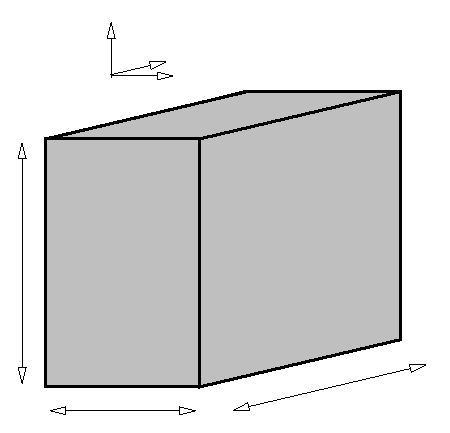
\includegraphics[width=4cm]{digue_perspective.eps}}
    \put(-0.5,4){(b)}
    \put(1.8,3.55){\tiny $\vec{e}_x$}
    \put(1.9,4.){\tiny $\vec{e}_y$}
    \put(1.1,4.2){\tiny $\vec{e}_z$}
    \put(0.2,1.9){\small $h$}
    \put(1.3,0.1){\small $L$}
    \put(3.6,0.4){\small $l$}
    \end{picture}
  \end{tabular}
  \caption{(a) Digue vue en coupe dans le plan $(\vec{e}_x,
    \vec{z})$. (b) Digue vue en perspective.}
  \label{fig:digue}
\end{figure}

%%%%%%%%%%%%%%%%%%%%%%%%%%%%%%%%%%%%%%%%%%%%%%%%%%%%%%%%%%%%%%%%%%%%%%%%%%%%%%%
\subsection{Cylindre immerg\'e dans deux fluides non miscibles}
%%%%%%%%%%%%%%%%%%%%%%%%%%%%%%%%%%%%%%%%%%%%%%%%%%%%%%%%%%%%%%%%%%%%%%%%%%%%%%%

\noindent
Un solide assimilable \`a un cylindre de section $S$ et de hauteur $H$,
de masse volumique $\rho_c$ est immerg\'e dans un r\'ecipient contenant
deux liquides non miscibles homog\`enes de masses volumiques constantes
$\rho_1$ et $\rho_2$.
On rep\`ere la position du cylindre par l'altitude $z$ de sa partie
sup\'erieure par rapport \`a l'interface (figure~\ref{fig:glacon}a).

Ecrire l'\'equation permettant de d\'eterminer la position d'\'equilibre $z_0$
du cylindre \`a l'interface entre les deux fluides
et discuter l'existence d'une position d'\'equilibre et sa stabilit\'e.

\begin{figure}[htb]
\begin{center}
\input{../FIGURES/cyl-misc.pstex_t} \qquad \input{../FIGURES/glacon.pstex_t}
\end{center}
\caption{Cylindre en \'equilibre \`a l'interface entre deux fluides non
miscibles (a). Gla\c{c}on flottant \`a la surface d'un verre d'eau (b).}
\label{fig:glacon}
\end{figure}

%%%%%%%%%%%%%%%%%%%%%%%%%%%%%%%%%%%%%%%%%%%%%%%%%%%%%%%%%%%%%%%%%%%%%%%%%%%%%%%
\subsection{Fonte d'un gla\c{c}on}
%%%%%%%%%%%%%%%%%%%%%%%%%%%%%%%%%%%%%%%%%%%%%%%%%%%%%%%%%%%%%%%%%%%%%%%%%%%%%%%

Un gla\c{c}on est en \'equilibre \`a la surface d'un verre d'eau 
compl\`etement rempli (figure~\ref{fig:glacon}b).
En utilisant le principe de conservation de la masse et le th\'eor\`eme
d'Archim\`ede, d\'eterminer le niveau d'eau dans le verre une fois
le gla\c{c}on fondu.
Le verre d\'eborde-t'il ?


%%%%%%%%%%%%%%%%%%%%%%%%%%%%%%%%%%%%%%%%%%%%%%%%%%%%%%%%%%%%%%%%%%%%%%%%%%%%%%%
\subsection{Stabilit\'e d'un bateau}
%%%%%%%%%%%%%%%%%%%%%%%%%%%%%%%%%%%%%%%%%%%%%%%%%%%%%%%%%%%%%%%%%%%%%%%%%%%%%%%



Lorsqu'un bateau est \'ecart\'e de sa position d'\'equilibre, il subit
de la part du poids et de la pouss\'ee d'Archim\`ede un couple qui
peut soit le redresser et le ramener \`a sa position d'\'equilibre
(que l'on qualifie alors de stable), soit le faire chavirer
(\'equilibre instable).
\begin{figure}[htbp]
  \centering
  \begin{tabular}{cc}
    \begin{picture}(6,3)(0,0)
    \put(0,3){(a)}
    \put(0,0){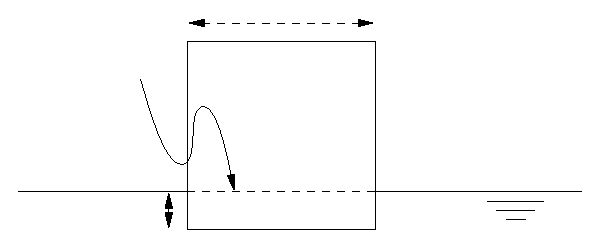
\includegraphics[width=6cm]{stable_equilibre.eps}}
    \put(1.2,0.1){$h$}
    \put(0.0,2.1){\small \textit{Ligne de}}
    \put(0.0,1.7){\small \textit{flottaison}}
    \put(2.6,2.5){$L$}
    \end{picture} &
    \begin{picture}(6,3)(0,0.15)
    \put(0,3.15){(b)}
    \put(0,0){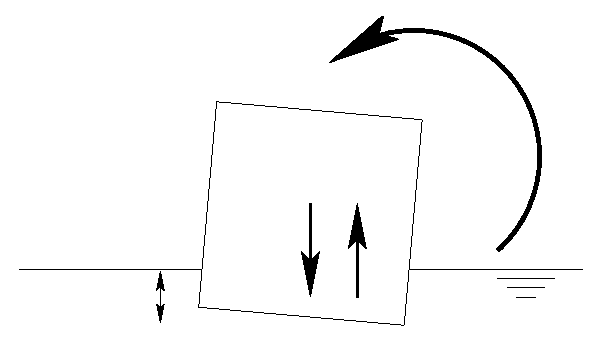
\includegraphics[width=5.5cm]{stable_gitee.eps}}
    \put(0.9,0.2){$h$}
    \put(2.2,0.5){$\vec{P}$}
    \put(3.3,0.5){$\vec{R}$}
    \put(4.0,3){\textit{Couple de}}
    \put(4.8,2.5){\textit{redressement}}
    \end{picture} \\
    \begin{picture}(6,4)(0,0)
    \put(0,3){(c)}
    \put(0,0){\includegraphics[width=6cm]{instable_equilibre.eps}}
    \put(1.0,0.3){$h$}
    \end{picture} &
    \begin{picture}(6,4)(0,0.25)
    \put(0,3.25){(d)}
    \put(0,0){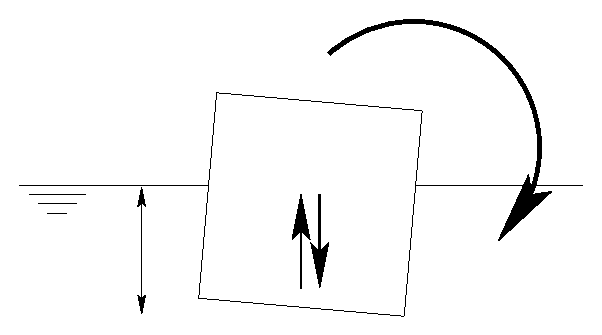
\includegraphics[width=5.5cm]{instable_gitee.eps}}
    \put(0.7,0.4){$h$}
    \put(2.2,0.5){$\vec{R}$}
    \put(3.1,0.5){$\vec{P}$}
    \put(4.0,3){\textit{Couple de}}
    \put(4.8,2.5){\textit{chavirement}}
    \end{picture}
  \end{tabular}
  \caption{(a) Configuration d'\'equilibre stable. Une fois git\'e (b), le bateau subit de la part du poids et de la pouss\'ee d'Archim\`ede un couple qui le ram\`ene \`a sa position d'\'equilibre. (c) Configuration instable. Une fois \'ecart\'e de sa position d'\'equilibre, l'action du poids et de la force d'Archim\`ede tend \`a faire chavirer le bateau.}
  \label{fig:equilibre}
\end{figure}

Dans cet exercice, on s'int\'eresse \`a la stabilit\'e d'un bateau
id\'ealis\'e sous la forme d'un carr\'e de densit\'e uniforme $\rho_b$. Le bateau d'ar\^ete $L$ est
immerg\'e sur une hauteur $h$, que l'on appelle le tirant d'eau. Le
rapport entre la masse volumique du bateau $\rho_b$ et celle du fluide
$\rho_f$ sera not\'ee $\beta$.

Dans un premier temps, la stabilit\'e de la position o\`u une ar\^ete
est horizontale est envisag\'ee.

\begin{enumerate}
\item Ecrire la condition d'\'equilibre du bateau et en d\'eduire une
  relation liant $\beta$, $h$ et $L$.
\item Calculer la position du centre de car\`ene $C$ et du centre de
  gravit\'e $G$.
\item Le bateau est tr\`es l\'eg\`erement git\'e d'un angle $\alpha$
  ($\alpha \ll 1$). Donner la position du nouveau centre de car\`ene $C'$.
\end{enumerate}
Pour \'etudier la stabilit\'e d'un \'equilibre, il est utile
d'introduire un point fictif appel\'e \textbf{m\'etacentre}, situ\'e
\`a l'intersection de $(CG)$ et d'une verticale passant par $C'$.

\begin{enumerate}
\setcounter{enumi}{3}
\item Calculer la distance $CM$ et v\'erifier qu'elle est bien \'egale
  \`a $I/W$, avec $I = \int_\mathrm{flottaison} x^2 \mathrm{d}S$ et
  $W$ est le volume de fluide d\'eplac\'e, encore appel\'e \textit{d\'eplacement}.
\item Discuter de la stabilit\'e du bateau en fonction de la position
  relative de $G$ et $M$.
\item En d\'eduire les valeurs de $\beta$ pour lesquelles cet
  \'equilibre est stable.

\item Refaire l'étude précédente dans le cas où le bateau
pr\'esente une diagonale horizontale.

 
\end{enumerate}
 \vspace{3cm}
\begin{figure}[htbp]
% 
  \centering
  \begin{picture}(6,5)(0,0)
  \put(0,0.5){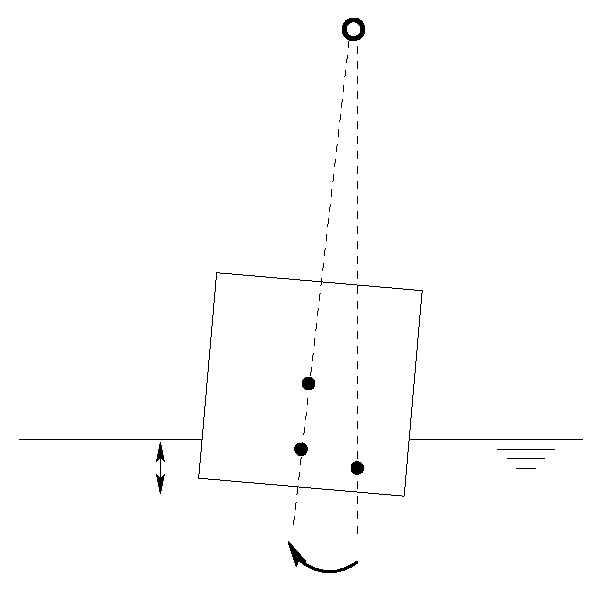
\includegraphics[width=6cm]{metacentre.eps}}
  \put(1.0,1.5){$h$}
  \put(2.5,1.7){$C$}
  \put(2.6,2.5){$G$}
  \put(3.7,1.7){$C'$}
  \put(3.1,0.2){$\alpha$}
  \put(2.9,6.2){$M$}
  \end{picture}
  \caption{Construction du m\'etacentre. Le bateau est \'ecart\'e de sa position d'\'equilibre d'un angle de g\^ite $\alpha$. Le m\'etacentre $M$ est situ\'e \`a l'intersection de $(CG)$ et de la verticale passant par $C'$.}
  \label{fig:metacentre}
\end{figure}

%On s'int\'eresse maintenant \`a la stabilit\'e de l'\'equilibre du
%bateau lorsque celui-ci 
%\begin{figure}[htbp]
%  \centering
%  \begin{picture}(6,3)(0,0)
%    \put(0,0){\includegraphics[width=6cm]{diagonale.eps}}
%    \put(1.1,0.4){$h$}
%  \end{picture}
%  \caption{Configuration o\`u le bateau pr\'esente une diagonale horizontale.}
%  \label{fig:diagonale}
%\end{figure}






\comment{
\begin{enumerate}
\setcounter{enumi}{6}
\item Ecrire \`a nouveau les conditions d'\'equilibre et trouver une
  relation connectant $\beta$, $h$ et $L$.
\item Trouver la position du centre de car\`ene et du centre de
  gravit\'e.
\item Donner la position du m\'etacentre. On pourra utiliser la
  relation $CM = I/W$.
\item En d\'eduire un ou plusieurs intervalles de $\beta$ pour lequel
  (lesquels) cet \'equilibre est stable.
\item Rasssemblez les r\'esultats des questions 6 et 10. Que se passe-t'il pour les valeurs de $\beta$ ne correspondant pas \`a ces questions ?
\end{enumerate}


 
%%%%%%%%%%%%%%%%%%%%%%%%%%%%%%%%%%%%%%%%%%%%%%%%%%%%%%%%%%%%%%%%%%%%%%%%%%%%%%%
\subsection{Force d'adh\'esion d'une goutte}
%%%%%%%%%%%%%%%%%%%%%%%%%%%%%%%%%%%%%%%%%%%%%%%%%%%%%%%%%%%%%%%%%%%%%%%%%%%%%%%

\noindent Deux surfaces mouill\'ees peuvent coller tr\`es fortement
ensemble si le liquide les mouille avec un angle de contact $\theta_c$
inf\'erieur \`a un angle seuil $\theta_s$.

\noindent On \'ecrase une grosse goutte entre deux plaques distantes
de $H$. La goutte \'ecras\'ee forme ce que l'on appelle un
\textit{pont capillaire}, illustr\'e sur la figure~\ref{fig:goutte}.
Notons $R$ son rayon et $A \sim \pi R^2$ sa surface. La loi de Laplace
\begin{equation}
  \label{eq:laplace}
  \Delta p = \gamma \left( \frac{1}{R} + \frac{1}{R'} \right)
\end{equation}
va nous permettre d'\'evaluer la saut de pression \`a l'interface.

\begin{enumerate}
\item D\'eterminer la courbure $C = 1/R + 1/R'$ de la surface au
  niveau du point $M$.
\item En d\'eduire le saut de pression \`a l'interface en fonction de
  la tension superficielle $\gamma$, du rayon $R$, de l'angle de
  contact $\theta_c$ et de l'\'ecartement $H$ des plaques. Donner une
  estimation de ce saut dans la limite o\`u $R \gg H$. Dans toute la
  suite, on se place dans cette limite.
\item Donner la valeur limite $\theta_s$ de l'angle de contact \`a ne
  pas d\'epasser pour que cette force soit attractive.
\item Application num\'erique : \\ En prenant $R = 1\,\mathrm{cm}$, $H = 5\,
  \mu\mathrm{m}$, $\theta_c = 0$ et $\gamma~=~72\,\mathrm{mN/m}$ (tension superficielle de l'eau), donner une estimation de la
  d\'epression dans la goutte, ainsi que de la force d'adh\'esion
  r\'esultante. 

  \noindent On accroche maintenant un r\'ecipient \`a la plaque
  inf\'erieure. Quel volume d'eau la plaque peut-elle supporter
  gr\^ace \`a la force d'adh\'esion cr\'e\'ee par cette goutte ?
\end{enumerate}
\begin{figure}[htbp]
  \centering
  \begin{tabular}{c}
    \begin{picture}(8,4)(0,0)
    \put(0,0){\includegraphics[width=8cm]{goutte.eps}}
    \put(2.6,2.3){\small $\theta_c$}
    \put(5.6,1.7){\small $M$}
    \put(4.6,1.9){\small $R$}
    \put(6.8,1.7){\small $H$}
    \end{picture} 
  \end{tabular}
  \caption{Goutte coinc\'ee entre deux plaques et formant un pont capillaire.}
  \label{fig:goutte}
\end{figure}


%%%%%%%%%%%%%%%%%%%%%%%%%%%%%%%%%%%%%%%%%%%%%%%%%%%%%%%%%%%%%%%%%%%%%%%%%%%%%%%
\subsection{Pression dans deux fluides non miscibles}
%%%%%%%%%%%%%%%%%%%%%%%%%%%%%%%%%%%%%%%%%%%%%%%%%%%%%%%%%%%%%%%%%%%%%%%%%%%%%%%

Un r\'ecipient contient deux fluides non miscibles (par exemple de l'huile
et de l'eau) de masses volumiques respectives $\rho_1$ et $\rho_2$,
constantes (figure~\ref{fig:distrib}b).
La pression atmosph\'erique r\'egnant \`a l'ext\'erieur, not\'ee $P_a$,
est suppos\'ee constante. 
\begin{enumerate}
\item
D\'eterminer la distribution de pression $p_1(z)$ dans le liquide 1
($z\in[h, H]$) en fonction de $\rho_1$, $H$, $g$ et $P_a$.
\item
D\'eterminer la distribution de pression $p_2(z)$ dans le liquide 2
($z\in[0, h]$)
en fonction de $\rho_1$, $\rho_2$, $h$, $g$, $P_a$ et $e=H-h$.
\item
Calculer la r\'esultante des forces de pression exerc\'ees par les fluides
(air et liquides) sur le fond du r\'ecipient, de surface $S$.
Interpr\'eter le r\'esultat obtenu.
\end{enumerate}


%%%%%%%%%%%%%%%%%%%%%%%%%%%%%%%%%%%%%%%%%%%%%%%%%%%%%%%%%%%%%%%%%%%%%%%%%%%%%%%
\subsection{Efforts de pression sur un barrage}
%%%%%%%%%%%%%%%%%%%%%%%%%%%%%%%%%%%%%%%%%%%%%%%%%%%%%%%%%%%%%%%%%%%%%%%%%%%%%%%

\begin{figure}[htb]
\begin{center}
\input{../FIGURES/barrage.pstex_t} \qquad \input{../FIGURES/face.pstex_t}
\end{center}
\caption{Vues de profil (a) et de face (b) du barrage.}
\label{fig:barrage}
\end{figure}

\noindent
Un barrage constitu\'e d'une paroi verticale en $y=0$ et de largeur $2L$
retient une r\'eserve d'eau de hauteur $H$ (figure~\ref{fig:barrage}).
\begin{enumerate}
\item
D\'eterminer la r\'esultante des efforts de pression exerc\'es par les fluides
(eau et air) sur la paroi du barrage.
\item
La paroi verticale est susceptible de pivoter autour de l'axe $(I, \vec{e}_x)$
o\`u $I$ est le point d'altitude $H/2$ (cf figure).
Calculer le moment des efforts de pression en $I$.
Dans quel sens la paroi risque de pivoter ?
\item
Calculer le point d'application de la r\'esultante des forces de pression.
\end{enumerate}



%%%%%%%%%%%%%%%%%%%%%%%%%%%%%%%%%%%%%%%%%%%%%%%%%%%%%%%%%%%%%%%%%%%%%%%%%%%%%%%
\subsection{Tronc d'arbre flottant}
%%%%%%%%%%%%%%%%%%%%%%%%%%%%%%%%%%%%%%%%%%%%%%%%%%%%%%%%%%%%%%%%%%%%%%%%%%%%%%%

Consid\'erons un cylindre homogène de masse volumique $\rho_c$, de rayon $R$,
de longueur $L$, flottant horizontalement dans l'eau et immergé à mi-hauteur 
dans un liquide homogène de masse volumique $\rho_0$.
La surface libre du liquide est \`a la pression atmosph\'erique $P_a$.
On introduit un repère $(O, \vec e_x, \vec e_y,\vec e_z)$ où $O$ est le centre
de gravité du cylindre, $\vec e_x$ est aligné avec l'axe du cylindre,
et $\vec e_z$ est vertical et orienté vers le bas.
On appelle ${\cal S}_l$ et ${\cal S}_a$ les portions de la surface latérale 
situées dans l'eau et dans l'air.


\begin{figure}[htb]
\begin{center}
\input{../FIGURES/tronc1.pstex_t} \qquad \input{../FIGURES/tronc2.pstex_t}
\end{center}
\caption{Cylindre flottant : (a) Vue de profil, (b) shéma dans le plan médian,
et repère mobile associé à un point $M$ du tronc.}
\label{fig:statique}
\end{figure}

\begin{enumerate}
\item

\item
Calculer la distribution de pression $p(z)$ dans le fluide.
\item
Calculez la force de pression exercée par l'eau sur le cylindre.
\item 
Calculez la force de pression exercée par l'air sur le cylindre.
\item 
En déduire la force totale de poussée exercée sur le cylindre.
\item 
Retrouvez ce résultat avec le théorème d'Archimède.
\item Quelle doit être la masse volumique $\rho_c$ du cylindre pour
que la position immergée à mi-hauteur soit une position d'équilibre ?

\end{enumerate}



%%%%%%%%%%%%%%%%%%%%%%%%%%%%%%%%%%%%%%%%%%%%%%%%%%%%%%%%%%%%%%%%%%%%%%%%%%%%%%%
\subsection{Equilibre d'un cylindre dans un fluide stratifi\'e}
%%%%%%%%%%%%%%%%%%%%%%%%%%%%%%%%%%%%%%%%%%%%%%%%%%%%%%%%%%%%%%%%%%%%%%%%%%%%%%%

Consid\'erons un cylindre de masse volumique $\rho_c$, de rayon $R$,
de hauteur $H$, compl\`etement immerg\'e dans un liquide de masse volumique
\textit{variable} $\rho(z) = \rho_0 (1 + \alpha z)$ o\`u $\rho_0$ et $\alpha$
sont des constantes.
La surface libre du liquide est \`a la pression atmosph\'erique $P_a$
(cf figure~\ref{fig:statique}).

\begin{figure}[htb]
\begin{center}
\input{../FIGURES/cylindre.pstex_t} \qquad \input{../FIGURES/section.pstex_t}
\end{center}
\caption{Vue de profil (a) et de dessous (b).
$\vec{n}_0$, $\vec{n}_1$ et $\vec{n}_2$ d\'esignent respectivement
les normales sortantes des surfaces $S_0$, $S_1$ et $S_2$ du cylindre.}
\label{fig:statique}
\end{figure}

\begin{enumerate}
\item
Quelle est la dimension de $\alpha$ ?
\item
Calculer la distribution de pression $p(z)$ dans le fluide.
\item
La surface sup\'erieure $S_1$ du cylindre \'etant \`a la profondeur $z$,
calculer :
\begin{enumerate}
\item
la r\'esultante des efforts de pression $\vec{F}_1$
exerc\'es par le fluide sur la surface $S_1$ du cylindre,
\item
la r\'esultante des efforts de pression $\vec{F}_2$
exerc\'es par le fluide sur la surface inf\'erieure $S_2$ du cylindre.
\item
Montrer que la r\'esultante des efforts de pression $\vec{F}_0$
exerc\'es par le fluide sur la surface lat\'erale $S_0$ du cylindre est nulle.
\item
Donner alors l'expression de la r\'esultante totale des efforts de pression 
$\vec{F}$ sur tout le cylindre.
\end{enumerate}
\item
Calculer le poids du fluide d\'eplac\'e par le cylindre.
Pouvait-on pr\'evoir ce r\'esultat ?
\item
D\'eterminer la position d'\'equilibre $z_0$ du cylindre.
Quelle condition doit v\'erifier $\rho_c$ pour que le cylindre \`a 
l'\'equilibre soit compl\`etement immerg\'e ?
\item
On perturbe la position verticale du cylindre pour l'amener en
$z_0 + \varepsilon$. 
\begin{enumerate}
\item
Calculer la r\'esultante des forces s'exer\c{c}ant sur le cylindre.
\item
Conclure sur la stabilit\'e de la position d'\'equilibre $z_0$ en fonction
du signe de $\alpha$.
\end{enumerate}
\end{enumerate}

}
}
